\documentclass{standalone}
\usepackage{tikz}
\usetikzlibrary{patterns, positioning}
\usepackage[sfdefault]{ClearSans} %% option 'sfdefault' activates Clear Sans as the default text font
\usepackage[T1]{fontenc}

\begin{document}
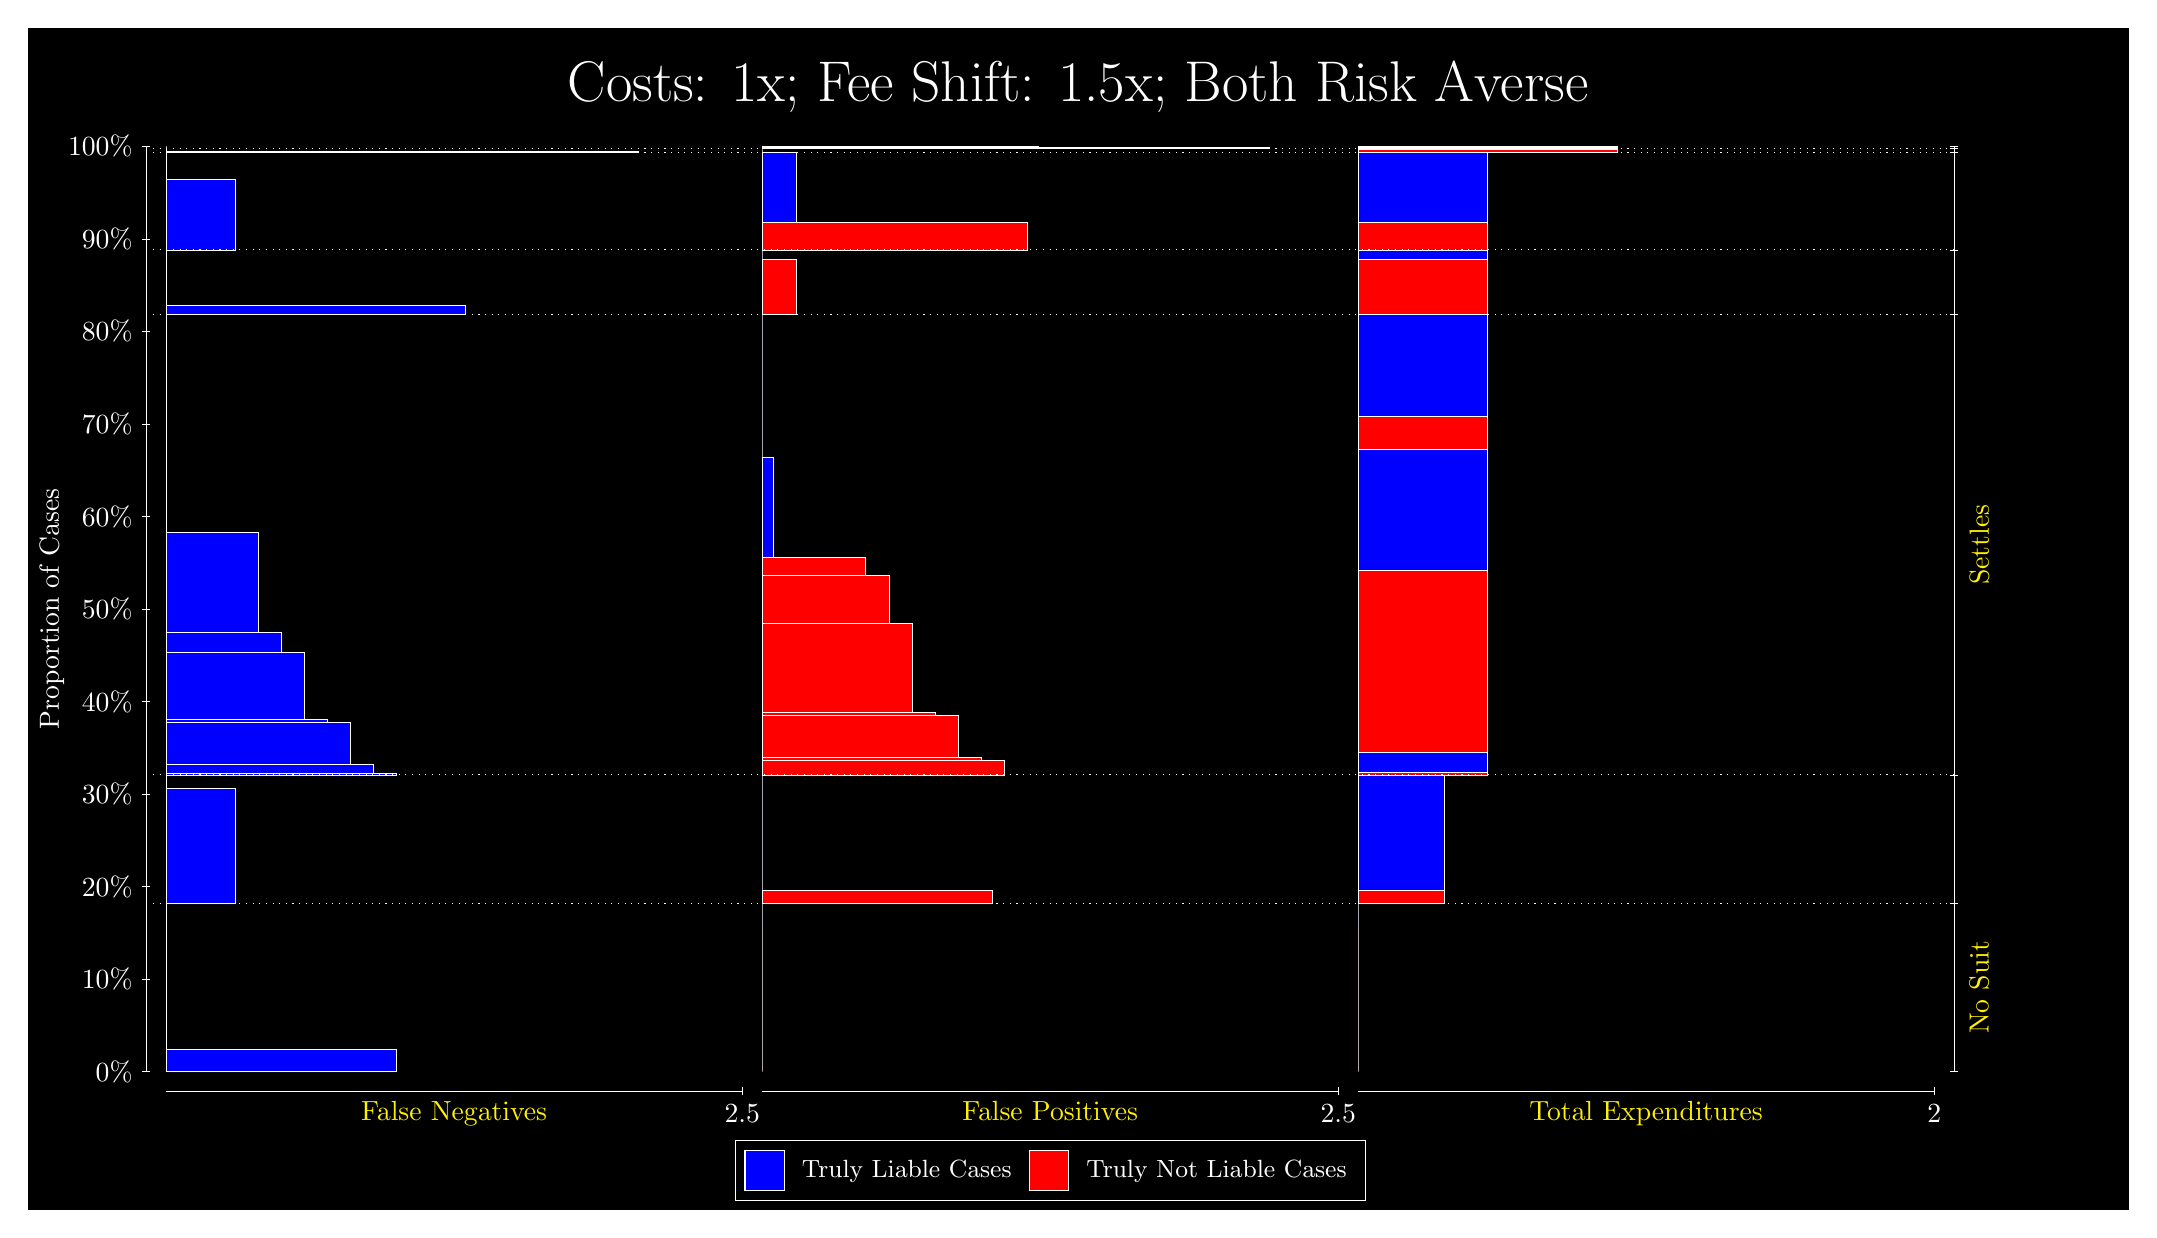
\begin{tikzpicture}
\draw[fill=black] (0,0) rectangle (26.667,15);
\draw[text=white] (0,13.5) rectangle (26.667,15) node[midway] {\huge Costs: 1x; Fee Shift: 1.5x; Both Risk Averse};
\draw[white, very thin] (1.5,1.75) -- (1.5,13.5);
\node[rotate=90, text=white, anchor=center] at (0.3, 7.625) {Proportion of Cases};
\draw[white, very thin] (1.45,1.75) -- (1.55,1.75);
\node[text=white, anchor=east] at (1.45, 1.75) {0\%};
\draw[white, very thin] (1.45,2.925) -- (1.55,2.925);
\node[text=white, anchor=east] at (1.45, 2.925) {10\%};
\draw[white, very thin] (1.45,4.1) -- (1.55,4.1);
\node[text=white, anchor=east] at (1.45, 4.1) {20\%};
\draw[white, very thin] (1.45,5.275) -- (1.55,5.275);
\node[text=white, anchor=east] at (1.45, 5.275) {30\%};
\draw[white, very thin] (1.45,6.45) -- (1.55,6.45);
\node[text=white, anchor=east] at (1.45, 6.45) {40\%};
\draw[white, very thin] (1.45,7.625) -- (1.55,7.625);
\node[text=white, anchor=east] at (1.45, 7.625) {50\%};
\draw[white, very thin] (1.45,8.8) -- (1.55,8.8);
\node[text=white, anchor=east] at (1.45, 8.8) {60\%};
\draw[white, very thin] (1.45,9.975) -- (1.55,9.975);
\node[text=white, anchor=east] at (1.45, 9.975) {70\%};
\draw[white, very thin] (1.45,11.15) -- (1.55,11.15);
\node[text=white, anchor=east] at (1.45, 11.15) {80\%};
\draw[white, very thin] (1.45,12.325) -- (1.55,12.325);
\node[text=white, anchor=east] at (1.45, 12.325) {90\%};
\draw[white, very thin] (1.45,13.5) -- (1.55,13.5);
\node[text=white, anchor=east] at (1.45, 13.5) {100\%};

\draw[white, very thin] (24.457,1.75) -- (24.457,13.5);
\draw[white, very thin] (24.407,1.75) -- (24.507,1.75);
\node[anchor=west] at (24.407, 1.75) {};
\draw[white, very thin] (24.407,3.886) -- (24.507,3.886);
\node[anchor=west] at (24.407, 3.886) {};
\draw[white, very thin] (24.407,5.5178) -- (24.507,5.5178);
\node[anchor=west] at (24.407, 5.5178) {};
\draw[white, very thin] (24.407,11.362) -- (24.507,11.362);
\node[anchor=west] at (24.407, 11.362) {};
\draw[white, very thin] (24.407,12.184) -- (24.507,12.184);
\node[anchor=west] at (24.407, 12.184) {};
\draw[white, very thin] (24.407,13.427) -- (24.507,13.427);
\node[anchor=west] at (24.407, 13.427) {};
\draw[white, very thin] (24.407,13.473) -- (24.507,13.473);
\node[anchor=west] at (24.407, 13.473) {};
\draw[white, very thin] (24.407,13.5) -- (24.507,13.5);
\node[anchor=west] at (24.407, 13.5) {};

\draw[white, very thin, fill=blue] (1.75,1.75) rectangle (4.6775,2.037);
\draw[white, very thin, fill=red] (1.75,2.037) rectangle (1.75,3.886);
\draw[white, very thin, fill=blue] (1.75,3.886) rectangle (2.6283,5.3492);
\draw[white, very thin, fill=red] (1.75,5.3492) rectangle (1.75,5.5178);
\draw[white, very thin, fill=blue] (1.75,5.5178) rectangle (4.6775,5.5369);
\draw[white, very thin, fill=blue] (1.75,5.5369) rectangle (4.3848,5.6482);
\draw[white, very thin, fill=blue] (1.75,5.6482) rectangle (4.092,6.1858);
\draw[white, very thin, fill=blue] (1.75,6.1858) rectangle (3.7993,6.2189);
\draw[white, very thin, fill=blue] (1.75,6.2189) rectangle (3.5065,7.0782);
\draw[white, very thin, fill=blue] (1.75,7.0782) rectangle (3.2138,7.3259);
\draw[white, very thin, fill=blue] (1.75,7.3259) rectangle (2.921,8.6006);
\draw[white, very thin, fill=red] (1.75,8.6006) rectangle (1.75,11.362);
\draw[white, very thin, fill=blue] (1.75,11.362) rectangle (5.5558,11.484);
\draw[white, very thin, fill=red] (1.75,11.484) rectangle (1.75,12.184);
\draw[white, very thin, fill=blue] (1.75,12.184) rectangle (2.6283,13.076);
\draw[white, very thin, fill=red] (1.75,13.076) rectangle (1.75,13.427);
\draw[white, very thin, fill=blue] (1.75,13.427) rectangle (7.7515,13.439);
\draw[white, very thin, fill=red] (1.75,13.439) rectangle (1.75,13.473);
\draw[white, very thin, fill=red] (1.75,13.473) rectangle (1.75,13.485);
\draw[white, very thin, fill=blue] (1.75,13.485) rectangle (1.75,13.5);
\draw[white, very thin, fill=red] (9.3189,1.75) rectangle (9.3189,3.599);
\draw[white, very thin, fill=blue] (9.3189,3.599) rectangle (9.3189,3.886);
\draw[white, very thin, fill=red] (9.3189,3.886) rectangle (12.246,4.0546);
\draw[white, very thin, fill=blue] (9.3189,4.0546) rectangle (9.3189,5.5178);
\draw[white, very thin, fill=red] (9.3189,5.5178) rectangle (12.393,5.7);
\draw[white, very thin, fill=red] (9.3189,5.7) rectangle (12.1,5.7347);
\draw[white, very thin, fill=red] (9.3189,5.7347) rectangle (11.807,6.2723);
\draw[white, very thin, fill=red] (9.3189,6.2723) rectangle (11.515,6.3136);
\draw[white, very thin, fill=red] (9.3189,6.3136) rectangle (11.222,7.4372);
\draw[white, very thin, fill=red] (9.3189,7.4372) rectangle (10.929,8.0505);
\draw[white, very thin, fill=red] (9.3189,8.0505) rectangle (10.636,8.2789);
\draw[white, very thin, fill=blue] (9.3189,8.2789) rectangle (9.4652,9.5536);
\draw[white, very thin, fill=blue] (9.3189,9.5536) rectangle (9.3189,11.362);
\draw[white, very thin, fill=red] (9.3189,11.362) rectangle (9.758,12.062);
\draw[white, very thin, fill=blue] (9.3189,12.062) rectangle (9.3189,12.184);
\draw[white, very thin, fill=red] (9.3189,12.184) rectangle (12.686,12.535);
\draw[white, very thin, fill=blue] (9.3189,12.535) rectangle (9.758,13.427);
\draw[white, very thin, fill=red] (9.3189,13.427) rectangle (9.3189,13.461);
\draw[white, very thin, fill=blue] (9.3189,13.461) rectangle (9.3189,13.473);
\draw[white, very thin, fill=red] (9.3189,13.473) rectangle (15.759,13.485);
\draw[white, very thin, fill=blue] (9.3189,13.485) rectangle (12.832,13.5);
\draw[white, very thin, fill=red] (16.888,1.75) rectangle (16.888,3.599);
\draw[white, very thin, fill=blue] (16.888,3.599) rectangle (16.888,3.886);
\draw[white, very thin, fill=red] (16.888,3.886) rectangle (17.986,4.0546);
\draw[white, very thin, fill=blue] (16.888,4.0546) rectangle (17.986,5.5178);
\draw[white, very thin, fill=red] (16.888,5.5178) rectangle (18.534,5.5525);
\draw[white, very thin, fill=blue] (16.888,5.5525) rectangle (18.534,5.8002);
\draw[white, very thin, fill=red] (16.888,5.8002) rectangle (18.534,8.116);
\draw[white, very thin, fill=blue] (16.888,8.116) rectangle (18.534,9.6573);
\draw[white, very thin, fill=red] (16.888,9.6573) rectangle (18.534,10.068);
\draw[white, very thin, fill=blue] (16.888,10.068) rectangle (18.534,11.362);
\draw[white, very thin, fill=red] (16.888,11.362) rectangle (18.534,12.062);
\draw[white, very thin, fill=blue] (16.888,12.062) rectangle (18.534,12.184);
\draw[white, very thin, fill=red] (16.888,12.184) rectangle (18.534,12.535);
\draw[white, very thin, fill=blue] (16.888,12.535) rectangle (18.534,13.427);
\draw[white, very thin, fill=red] (16.888,13.427) rectangle (20.181,13.461);
\draw[white, very thin, fill=blue] (16.888,13.461) rectangle (20.181,13.473);
\draw[white, very thin, fill=red] (16.888,13.473) rectangle (20.181,13.485);
\draw[white, very thin, fill=blue] (16.888,13.485) rectangle (20.181,13.5);
\draw[white, dotted] (1.5,3.886) -- (24.457,3.886);
\draw[white, dotted] (1.5,5.5178) -- (24.457,5.5178);
\draw[white, dotted] (1.5,11.362) -- (24.457,11.362);
\draw[white, dotted] (1.5,12.184) -- (24.457,12.184);
\draw[white, dotted] (1.5,13.427) -- (24.457,13.427);
\draw[white, dotted] (1.5,13.473) -- (24.457,13.473);
\draw[white, very thin] (1.75,1.5) -- (9.0689,1.5);
\node[text=yellow, anchor=north] at (5.4094, 1.5) {False Negatives};
\draw[white, very thin] (9.0689,1.45) -- (9.0689,1.55);
\node[text=white, anchor=north] at (9.0689, 1.45) {2.5};

\draw[white, very thin] (9.3189,1.5) -- (16.638,1.5);
\node[text=yellow, anchor=north] at (12.978, 1.5) {False Positives};
\draw[white, very thin] (16.638,1.45) -- (16.638,1.55);
\node[text=white, anchor=north] at (16.638, 1.45) {2.5};

\draw[white, very thin] (16.888,1.5) -- (24.207,1.5);
\node[text=yellow, anchor=north] at (20.547, 1.5) {Total Expenditures};
\draw[white, very thin] (24.207,1.45) -- (24.207,1.55);
\node[text=white, anchor=north] at (24.207, 1.45) {2};

\node[text=yellow, centered, rotate=90] at (24.777, 2.818) {No Suit};

\node[text=yellow, centered, rotate=90] at (24.777, 8.4397) {Settles};





\draw (12.978300999999998,1.5) node[draw=none] (baseCoordinate) {};
\begin{scope}[align=center]
        \matrix[scale=0.5, draw=white, below=0.5cm of baseCoordinate, nodes={draw}, column sep=0.1cm]{
            \node[rectangle, draw, minimum width=0.5cm, minimum height=0.5cm, fill=blue] {}; &
            \node[draw=none, font=\small, text=white] (B) {Truly Liable Cases}; &
            \node[rectangle, draw, minimum width=0.5cm, minimum height=0.5cm, fill=red] {}; &
            \node[draw=none, font=\small, text=white] (B) {Truly Not Liable Cases}; \\
            };
\end{scope}

\end{tikzpicture}
\end{document}